\section{Softwareudvikling AKA Greger er dum}
\subsection{Projektstyring}
Under de første møder til projektet, blev det aftalt at projektet skulle planlægges ved hjælp af sprints fra Scrum og at der skulle holdes jævnlige Scrum møder.
\newline
Der blev i starten af projektet derfor lavet en product backlog, hvori der blev angivet over hvor lang tid, hver eneste funktionalitet ville tage at implementere. Denne product backlog kan ses i BILLAG.
\newline
Sprintene skulle defineres ud fra, hvad der vil skabe mest værdi for projektet. Denne planlægning var tiltænkt at man kunne tilpasse projektarbejdet i forhold til undervisningen bedre. Derudover skulle sprints også laves på baggrund, for først at løse kravene og derefter visse udvalgte sekundære funktionaliteter.
\newline
Efter en sprint var defineret, ville der blive oprettet en Sprint backlog, som skulle dokumentere hvor meget arbejde der blev lagt i en problemstilling, og hvor meget workload der var tilbage. Sprint backloggen skulle derfor opdateres løbende under den pågældende sprint Sprint backlog'en fra uge 47-49 kan ses i figur \ref{fig:4749}:
\begin{figure}[ht]
	\centering
	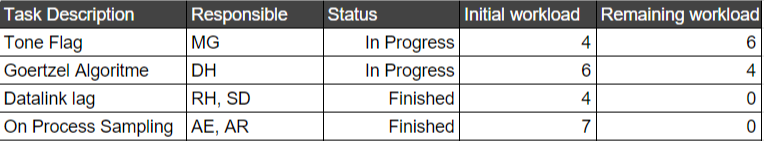
\includegraphics[width=15cm,height=25cm,keepaspectratio]{pictures/SprintBack47_49.png}
	\caption{Uge 47-49 sprint backlog}
	\label{fig:4749}
\end{figure}
\hfill \break

Yderlige eksempler på Sprint backlogs kan findes i BILAG.
\newline
Til Scrum møderne blev der udspecificeret en klar plan for, hvordan møderne skulle foregå, og hvilke elementer der skulle gennemgåes under møderne. I denne plan blev der også skrevet et kort teori afsnit, omkring hvordan man skal forholde sig til både Scrum møder og backlogs. Dette blev gjort med den hensigt, at hvert medlem ville være i stand til, at sikre at et Scrum møde blev udført korrekt og at backlogs blev opdateret.
\newline
Denne plan kan ses i BILLAG.

\subsection{Software Requirements Specification (SRS)}

\subsubsection{Idéudvikling}
Der blev i starten af projektet idéudviklet på den applikation der skulle laves. Der var flere idéer, hvorefter én blev valgt. Imellem disse idéer var en matematik applikation hvor en klient kunne sende et spørgsmål til en server og få et svar tilbage. Idéen var inspireret af Wolfram Alpha. Derudover var der også en idé, som til sidst blev valgt, som gik ud på at lave en chat applikation. Chat applikationen var inspireret af Skype, som fungerer på klient til klient plan. Der blev dog lagt op til at man kunne undersøge at lave en klient-server-klient hvis tiden var til det.
\hfill \break
Efter at have specificeret hvilken applikation der overordnet skulle laves, blev der lavet en brainstorm for krav til funktionaliteterne på applikationen, som kan ses på figur. 
\begin{figure}[ht]
	\centering
	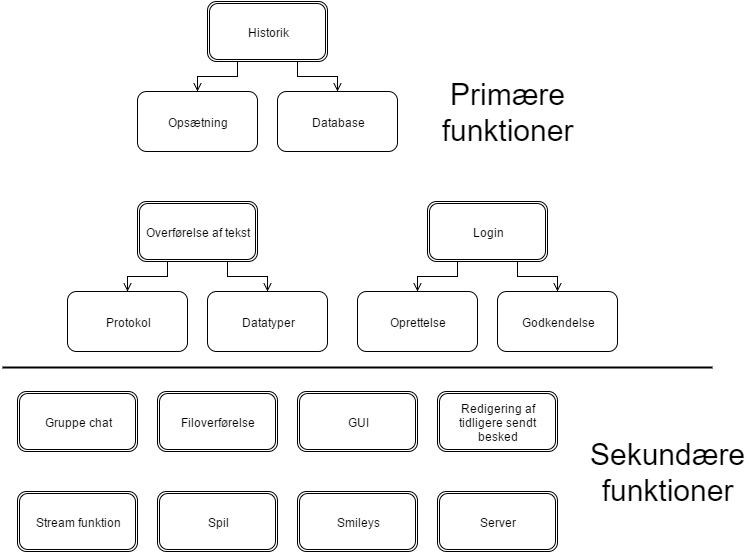
\includegraphics[width=15cm,height=25cm,keepaspectratio]{pictures/Ideudvikling.png}
	\caption{Brainstorm}
	\label{fig:brain}
\end{figure}
\newline
Som der ses på figur \ref{fig:brain} er funktionaliten delt op i to kategorier, primære- og sekundære funktioner. Hvor primære funktioner repræsenterer de funktionaliteter der minimum skal være i applikationen. De sekundære funktioner repræsenterer udvidelser som kan skabe værdi for brugeren.

\subsubsection{Kravspecifikation}
Udover at applikationen har nogle funktionaliteter, skal applikationen også have nogle krav. Disse krav er med til at opbygge applikationen og hjælper med at lede projektet mod en række problemstillinger der skal løses.
\newline
Kravene er som følger:
\begin{itemize}
	\item Sende beskeder mellem 2 applikationer
	\item Brugergrænseflade
	\item Pålidelig dataoverførsel
	\item Fejl testning af beskeder
	\item Se tidligere sendte og modtagede beskeder
	\item Login
\end{itemize}

\subsection{Softwareudvikling}
For at opbygge en velfungerende applikation,  er det imperativt at følge principperne indenfor softwareudvikling.

\subsubsection{Analyse fasen}
Der blev udarbejdet use cases, som viser hvordan brugeren interagerer med programmet, og som derudover hjælper til at afdække krav til applikation.
\newline
De use cases der blev udarbejdet var:
\begin{itemize}
	\item Login
	\item Historik
	\item Send besked
	\item Modtag besked
\end{itemize}
Use case over Send besked kan ses på figur HOMOSEXUEL og de resterende use cases kan findes i bilag BILLAG.
\hfill \break
Disse use cases blev brugt til at udarbejde en domænemodel, som kan ses i figur 
\begin{figure}[ht]
	\centering
	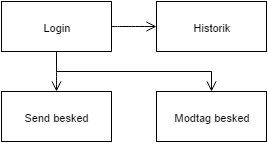
\includegraphics[width=10cm,height=10cm,keepaspectratio]{pictures/Domainmodel.png}
	\caption{Domænemodel}
	\label{fig:dom}
\end{figure}
\newline
Domæne modellen giver et simpelt indblik i hvordan applikationen skal fungere.
\hfill \newline
Udover at domæne modellen lægger op til at vi har som minimum fire klasser, blev det konstateret at der er behov for tre yderlige klasser, som opfylder følgende krav fra SRS, da de ikke blev afdækket af use casene: pålidelig dataoverførsel, brugergrænseflade og fejl testning af beskeder. Disse klasser blev midlertidigt navngivet \texttt{Fejlkontrol}, \texttt{UI} og \texttt{Levering}.

\subsubsection{Design klassen}
For at udarbejde et design klasse diagram blev der taget udgangspunkt i domænemodellen. Ved udvidelse og tilpasning af klasse diagrammet blev der anvendt design mønstre fra GRASP.
\newline
Jf. GRASP skal der være en controller, som er det første objekt efter en UI der modtager og koordinerer et systems operationer. Denne klasse bliver oprettet og snedigt kaldet Controller.
\newline
En skabelon for klasse diagrammet blev lavet, på baggrund af denne udvides og tilpasses den til et klasse diagram i en iterativ proces.
\begin{figure}[ht]
	\centering
	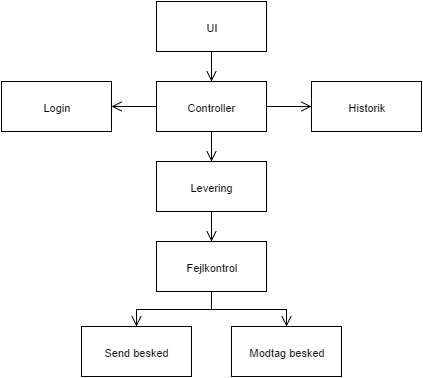
\includegraphics[width=10cm,height=10cm,keepaspectratio]{pictures/Flow.png}
	\caption{Flowmodel}
	\label{fig:flow}
\end{figure}
\newline
Under den iterative proces blev nogle meget generelle funktionaliteter undersøgt - hvordan man sender en besked og modtager en besked. Disse lagde op til nogle diskussioner og problemstillinger som diskuteres senere i rapporten. Grundet den iterative proces blev Send besked og Modtag besked omdybt til \texttt{Afspil} og \texttt{MyRecorder} for bedre at afspejle deres ansvarsområde. Jf. GRASPs principper havde disse klasser yderst lav kobling, men også lav cohesion grundet at der var mere ansvar i klasserne end de antydede. Derfor blev det konkluderet at disse ansvarsområder skulle deles op for at skabe højere cohesion. \texttt{Afspil} klassen havde ansvaret for at afspille toner, men ikke ansvaret for også at genererer toner. Derfor blev der lavet en information expert der påtog sig ansvaret at holde information omkring toner,netop klassen \texttt{Tone}. \texttt{MyRecorder} havde ligeledes kun et ansvar - at optage. Ansvaret for at analyserer optagelsen blev derfor tillagt en pure fabricated klasse ved navn \texttt{Goertzel}, for igen at øge cohesion.
\hfill \break

Senere i den iterative proces blev der draget inspiration fra datakommunikations lagdelte struktur - Open Systems Interconnection modellen (OSI). I denne model indgår der to lag, som afspejler klasserne Lervering- og Fejlkontrols ansvarsområde, nemlig: Datalinklaget(DLL) og Transportlaget. Klasse \texttt{Levering} er således blevet omdøbt til Transportlag, og \texttt{Fejlkontrol} er blevet omdøbt til \texttt{DLL}.
\newline
Grundet den iterative proces indeholdte DLL flere ansvarsområder end først forventet. Dette gjorde at man også her var nødsaget til at opdele ansvarsområdet. Der blev derfor pure fabricated en klasse, som ydede en service til DLL. Denne klasse fik navnet \texttt{CRC}, baseret på dens service.
\hfill \break
Disse udvidelser på klasse diagrammet skabte en ny problemstilling, de forskellige klasser snakker ikke i samme data format. Dataformaterne der snakkes i, er char strings, bit strings og tone chars.
\newline
Derfor blev der indført to klasser baseret over adapter pattern princippet, hvis formål var at oversætte dataformatet mellem de forskellige klasser. Adapter klasserne blev kaldt \texttt{CharDefinition} og \texttt{Tonekonvertering}.
\hfill \break
Efter projektets sidste iteration endtes der ud med et klasse diagram der kan ses på næste side.
\afterpage{\null\newpage}